\chapter{El teorema de Pitágoras}

Tal como hace Stillwell en su libro~\cite{MR2667826}, vamos a empezar el curso
con el teorema de Pitágoras. Es una buena elección: el teorema de Pitágoras es
uno de los teoremas más antiguos y además conecta varias ideas centrales en el
desarrollo de la matemática. 

La primera demostración rigurosa de este resultado se le atribuye conunmente a
Pitágoras, aunque no hay evidencia concreta de que Pitágoras haya encontrado
efectivamente una demostración.  El teorema ya era conocido en Babilonia muchos años 
antes del nacimiento de Pitágoras. Se sabe además que el teorema fue
descubierto independientemente en la matemática india y china, incluso
con demostraciones especiales para ciertos casos particulares. 

Deberíamos enunciar el teorema de Pitágoras sin apelar a la noción de longitud
de un segmento sino solamente a la de área, ya que en tiempos de Pitágoras los
matemáticos se sentían más cómodos con la noción de área que con la de
longitud.  De hecho, en aquellos tiempos, los matemáticos intentaban evitar
números irracionales ya que no podrían comprenderlos completamente. 
%\begin{example}
%	Supongamos que tenemos un triángulo rectángulo cuyos catetos miden $1$ y
%	$2$. El teorema de Pitágoras implica que la hipotenusa entonces mide
%	$\sqrt{5}$. El cuadrado de lados $\sqrt{5}$ tiene área igual a $5$ y para
%	calcular esto, gracias al teorema de Pitágoras, simplemente podemos hacer
%	\[
%		3\times3-2(2\times 1)=5.
%	\]
%\end{example}
\index{Teorema!de Pitágoras}
El \textbf{teorema de Pitágoras} es el siguiente:

\begin{theorem}[Pitágoras]
\index{Teorema!de Pitágoras}
Si $A$, $B$ y $C$ son los cuadrados de la figura~\ref{fig:pitagoras}, de
lados $a$, $b$ y $c$ respectivamente, entonces
$a^2+b^2=c^2$.
\end{theorem}

Vale también la afirmación recíproca: si $(a,b,c)$ es tal que $a^2+b^2=c^2$,
entonces existe un triángulo rectángulo de lados $a$ y $b$ e hipotenusa igual a
$c$. 

No sabemos cómo se demostró el teorema originalmente, se cree que fue mediante
manipulaciones de áreas. Se conocen muchas demostraciones del teorema de
Pitágoras, quizá casi cuatrocientas~\cite{loomis1968pythagorean}. 
En la página
\href{http://cut-the-knot.org/}{Cut the knot}, creada por Alexander Bogomolny, podremos
encontrar más de cien demostraciones, todas muy bien explicadas.  

%\begin{theorem}[Pitágoras]
%	Si $A$, $B$ y $C$ son los cuadrados de la figura~\ref{fig:pitagoras}, de
%	áreas $a$, $b$ y $c$ respectivamente, entonces
%	\[
%		a^2+b^2=c^2.
%	\]
%\end{theorem}
%
%\begin{proof}
%	Calculamos el área del cuadrado de la figura~\ref{fig:pitagoras} de dos
%	formas distintas y obtenemos que 
%	\[
%		4\frac{ab}{2}+c^2=(a+b)^2.
%	\]
%	Al simplificar esta expresión, $c^2=a^2+b^2$.
%\end{proof}

\begin{figure}
   \centering
   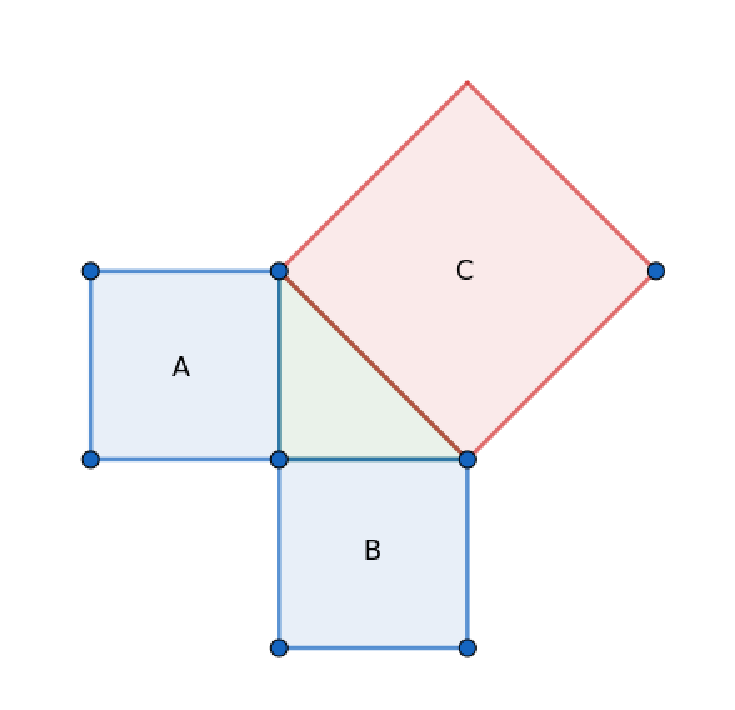
\includegraphics[scale=0.5]{images/thm_pitagoras}
   \caption{El teorema de Pitágoras.}
   \label{fig:pitagoras}
\end{figure}

\begin{exercise}
	Demuestre el teorema de Pitágoras utilizando el diagrama de la
	figura~\ref{fig:pitagoras1}.
	\begin{figure}[h]
		\centering
		\includegraphics[scale=.4]{images/pitagoras_proof}
		\caption{Otra demostración del teorema de Pitágoras, en general
		atribuida a la matemática china.}
		\label{fig:pitagoras1}
	\end{figure}
\end{exercise}

\begin{exercise}
	Utilice la figura~\ref{fig:semejanza} y 
	demuestre el teorema de Pitágoras.
	\begin{figure}[h]
		\centering
		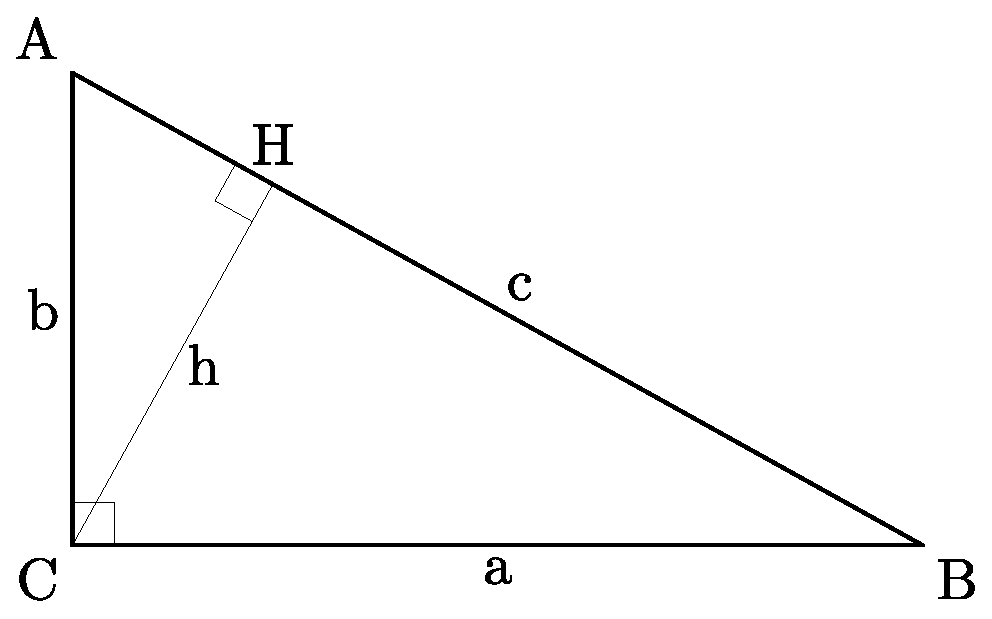
\includegraphics[scale=.2]{images/pitagoras_semejanza}
		\caption{Otra demostración del teorema de Pitágoras.}
		\label{fig:semejanza}
	\end{figure}
\end{exercise}

\begin{exercise}
	Utilice la figura~\ref{fig:Bhaskara} y 
	demuestre el teorema de Pitágoras.
	\begin{figure}[h]
		\centering
		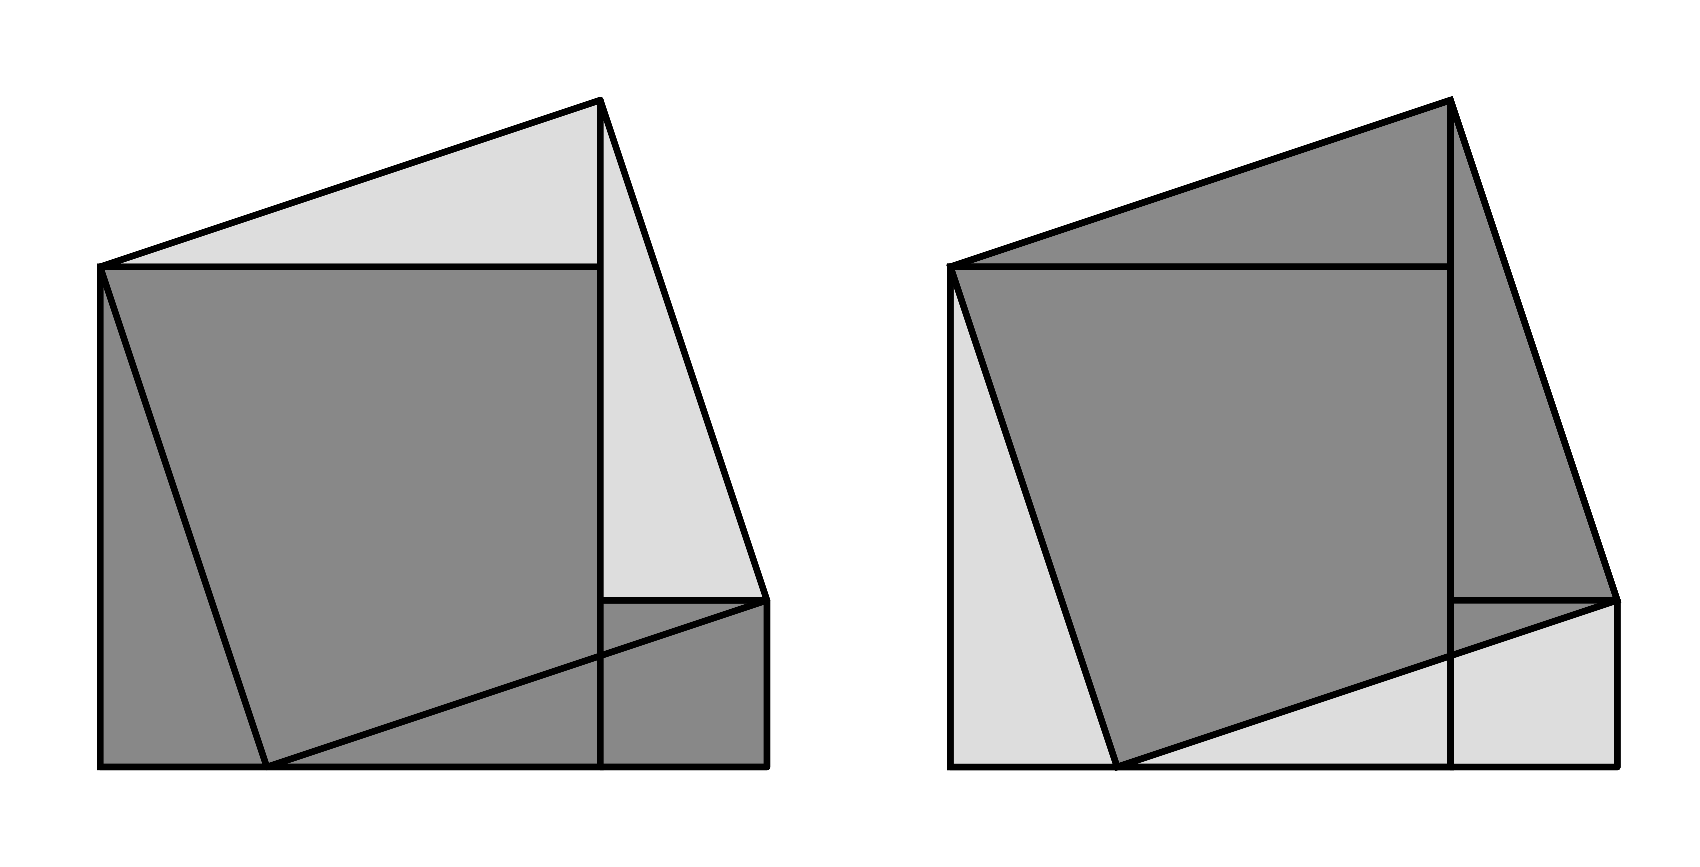
\includegraphics[scale=.2]{images/pitagoras_bhaskara}
		\caption{Otra demostración del teorema de Pitágoras, en general
		atribuida al matemático indio Bhaskara.}
		\label{fig:Bhaskara}
	\end{figure}
\end{exercise}


\begin{exercise}
	Utilice la figura~\ref{fig:arabe} y 
	demuestre el teorema de Pitágoras.
	\begin{figure}[h]
		\centering
		\includegraphics[scale=.5]{images/pitagoras_arabe}
		\caption{Otra demostración del teorema de Pitágoras, en general
		atribuida al matemático árabe Thabit ibn Qurrá.}
		\label{fig:arabe}
	\end{figure}
\end{exercise}

\begin{exercise}
	\index{Zhoubi Suanjing}
	Uno de los textos más antiguos de matemática china es el Zhoubi Suanjing,
	que data del período de la dinastía Zhou. Allí aparece una de las primeras
	demostraciones escritas del teorema de Pitágoras, basada en la
	figura~\ref{fig:China}. ¿Cómo puede usarse esa figura para demostrar el
	teorema de Pitágoras?
	\begin{figure}[h]
		\centering
		\includegraphics[scale=0.2]{images/pitagoras_china}
		\caption{Una demostración del teorema de Pitágoras.}
		\label{fig:China}
	\end{figure}
\end{exercise}

\begin{exercise}
	En los elementos de Euclides aparece una demostración del teorema de
	Pitágoras. ¿Cuál es esa demostración? ¿Aparecen otras demostraciones del
	teorema de Pitágoras en estos famosos libros de Euclides?
\end{exercise}

\begin{exercise}
	Existe una demostración del teorema de Pitagóras que se le atribuye a
	Leonardo Da Vinci. ¿Cuál es esa demostración?
\end{exercise}

\begin{exercise}
	La demostración del teorema de Pitágoras de este ejercicio fue descubierta
	por Garfield, el vigésimo Presidente de los Estados Unidos.  Demuestre el
	teorema de Pitágoras utilizando la figura~\ref{fig:garfield}.
	\begin{figure}[h]
		\centering
		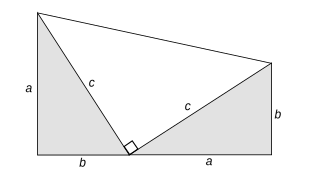
\includegraphics[scale=0.5]{images/garfield}
		\caption{La demostración de Garfield del teorema de Pitágoras.}
		\label{fig:garfield}
	\end{figure}
\end{exercise}


El teorema de Pitágoras sugiere sutilmente que existe una profunda relación
entre la aritmética y la geometría. Esta relación entre aritmética y geometría
es también fundamental en el desarollo de las matemáticas. 

Se cree que en tiempos antiguos se usaban distintas soluciones de la ecuación
del teorema de Pitágoras para construir ángulos rectos.  Por ejemplo, con una
cuerda con doce nudos equidistantes (es decir, una cuerda de ``longitud'' igual
a doce), se lograba construir el triángulo rectángulo $(3,4,5)$.  Hoy en día
usamos el teorema de Pitágoras para calcular longitudes y distancias.  Si
$A=(a_1,a_2)$ y $B=(b_1,b_2)$ son dos puntos del plano cartesiano, se define la
distancia entre $A$ y $B$ como 
\[
	\dist(A,B)=\sqrt{(a_1-b_1)^2+(a_2-b_2)^2}.
\]
Esta fórmula para calcular la distancia entre dos puntos del plano puede
extenderse fácilmente a puntos de un espacio de dimensión finita arbitraria. 

Se tiene
además una generalización del teorema de Pitágoras a espacios vectoriales de
dimensión finita: Si $V$ es un espacio vectorial con producto interno y
$v_1,\dots,v_n\in V$ son vectores ortogonales dos a dos, entonces 
\[
	\|v_1+\cdots+v_n\|^2=\sum_{i=1}^n \|v_i\|^2.
\]
Se recupera el teorema de Pitágoras al tomar $V=\R^2$ con el producto interno
usual.
%\[
%	\langle (x_1,y_1),(x_2,y_2)\rangle=x_1x_2+y_1y_2.
%\]

\begin{figure}[h]
	\centering
	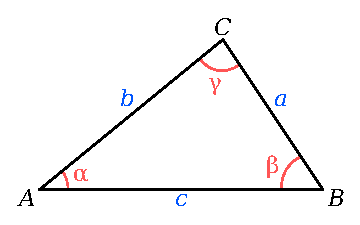
\includegraphics[scale=.5]{images/coseno}
	\caption{El teorema del coseno.}
	\label{fig:coseno}
\end{figure}

El teorema de Pitágoras puede verse como un caso particular del \textbf{teorema
del coseno}, que afirma que en un triángulo como el que vemos en la
figura~\ref{fig:coseno}, se tiene $c^2=a^2+b^2-2ab\cos\gamma$.

\begin{exercise}
	Demuestre el teorema del coseno.
\end{exercise}

Con el teorema del coseno podemos demostrar un lindo resultado publicado por el
matemático escocés Matthew Stewart en 1746: Si se tiene un triángulo como el
que vemos en la figura~\ref{fig:Stewart}, entonces
\[
	mb^2+nc^2=mn^2+nm^2+ad^2.
\]

\begin{figure}[h]
	\centering
	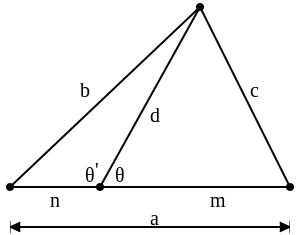
\includegraphics[scale=.4]{images/stewart}
	\caption{El teorema de Stewart.}
	\label{fig:Stewart}
\end{figure}

Aparentemente Stewart publicó este resultado en 1746 cuando era candidato a
reemplazar a Maclaurin como profesor de la Universidad de Edimburgo.  Se cree
que Arquímedes conocía ya este resultado. De hecho, el teorema de Stewart es
una generalización del teorema de las medianas de Apolonio, que afirma 
que en el triángulo de la figura~\ref{fig:Stewart} se tiene
\[
	b^2+c^2=\frac12a^2+2d^2.
\]

\begin{exercise}
	Demuestre el teorema de Stewart.
\end{exercise}

\begin{exercise}
	Demuestre el teorema de las medianas de Apolonio.
\end{exercise}

\section*{Ternas pitagóricas}
\index{Ternas pitagóricas}

Nos proponemos ahora encontrar ternas pitagóricas, es decir ternas
$(a,b,c)\in\N^3$ tales que $a^2+b^2=c^2$.  Para más información sobre aspectos
históricos sobre la construcción de ternas pitagóricas conviene mirar el
segundo volumen del tratado de Dickson sobre la historia de la teoría de
números~\cite{MR0245500}. 

\begin{exercise}
	Si $(a,b,c)$ es una terna pitagórica, entonces $(ka,kb,kc)$
	es una terna pitagórica.
\end{exercise}

\index{Terna pitagórica!primitiva}
Un ejemplo fácil de terna
pitagórica es $(3,4,5)$. 
Otro ejemplo de terna pitagórica es $(6,8,10)$, aunque podríamos acusarlo de no
es muy interesante pues puede obtenerse como 
\[
(6,8,10)=2\times (3,4,5). 
\]
Nos interesan entonces las ternas pitagóricas
\textbf{primitivas}, es decir las ternas pitagóricas $(a,b,c)$ con $a$, $b$ y $c$
coprimos. Veamos otros ejemplos de ternas pitagóricas primitivas:
\begin{align*}
	(5,12,13), &&
	(8,15,17), &&
	(7,24,25), && 
	(20,21,29),&&
	(12,35,37), \\
	(9,40,41), &&
	(28,45,53),&&
	(11,60,61),&&
	(16, 63, 65),&&
	(33, 56, 65),\\
	(48, 55, 73),&&
	(13, 84, 85),&&
	(36, 77, 85),&&
	(39, 80, 89),&&
	(65, 72, 97).
\end{align*}

Si bien Pitágoras vivió alrededor del 500 a. C., las ternas pitagóricas se
conocen desde mucho antes. Se sabe que las ternas pitagóricas fueron de interés
en Babilonia, en China y en India, se cree que para la construccción de ángulos
rectos.  Una de las referencias más antiguas a las ternas pitagóricas es una
tabla babilónica de arcilla conocida como Plimpton 322. Se cree que esta tabla
fue escrita en el año 1800 a. C. El nombre se debe al siguiente hecho: a
comienzos del siglo XX un editor llamado George Arthur Plimpton compró aquella
tabla de barro y tiempo después la entregó a la Universidad de Columbia; esta
tabla es la número 322 de la colección que Plimpton cedió a la Universidad de
Columbia.  Existen diversas interpretaciones sobre qué información contiene
esta tabla y cómo fue que los babilónicos pudieron calcularla. 

%Consideremos la figura\dots 
%Claramente tenemos $BC=AD$. Si $a+b$ es el lado $AC$, entonces $DB=a-b$. 
%Observemos además que
%\[
%	AO=OC=\frac12(a+b),\quad
%	DO=OB=\frac12(a-b)
%\]
%y entonces $AB=AO+OB$ y $AD=AO-OD$. Si elevamos al cuadrado, 
%\[
%	(a+b)^2=AE,\quad
%	(a-b)^2=FG
%

Un estudio reciente revela que la tabla describe las formas del triángulo
rectángulo usando una novedosa forma de trigonometría; para más información
referimos a~\cite{MR3716328}.

\begin{figure}
   \centering
   \includegraphics[scale=0.8]{images/plimpton322}
   \caption{La tabla Plimpton 322.}
   \label{fig:plimpton}
\end{figure}


Según Proclo, Pitágoras conocía la regla 
\[
	x=2\alpha+1,\quad
	y=2\alpha^2+2\alpha,\quad
	z=y+1,
\]
para generar ternas pitagóricas. Platón conocía la regla 
\[
	x=2\alpha,\quad
	y=\alpha^2-1,\quad
	z=\alpha^2+1.
\]
En sus elementos, en la proposición 5 del libro II, Euclides dio la regla 
\[
		x=\alpha\beta\gamma,
		\quad
		y=\frac12\alpha(\beta^2-\gamma^2),
		\quad
		z=\frac12\alpha(\beta^2+\gamma^2),
\]
para construir ternas pitagóricas.  En la proposición 30 del libro X, dio otra
regla:
\[
		x=\sqrt{mn},\quad
		y=\frac12(m-n),\quad
		z=\frac12(m+n).
\]
Al menos un siglo antes que Diofanto, Nipsus dio la siguiente regla: 
\begin{align*}
	&z=\frac12(x^2+1), && y=\frac12(x^2-1), &&\text{si $x$ es impar},\\
	&z=\frac14x^2+1, && y=\frac14x^2-1, &&\text{si $x$ es par},
\end{align*}
y además $x^2=z^2-y^2$. Estas fórmulas son equivalentes a las fórmulas dadas
por Pitágoras y Platón. Más tarde, Diofanto presentó un ingenioso método
geométrico que le permitió obtener las siguientes fórmulas 
\begin{equation}
	\label{eq:formula}
	a=(p^2-q^2)r,\quad
	b=2pqr,\quad
	c=(p^2+q^2)r,
\end{equation}
para generar ternas pitagóricas. 

Los babilónicos no disponía de notación algebraica, pero se cree que 
conocían  
las fórmulas~\eqref{eq:formula} en el caso $r=1$ y que así fue como lograron
listar ternas pitagóricas. Las fórmulas~\eqref{eq:formula} como método para
obtener ternas pitagóricas aparece también en la matemática india y en
manuscritos árabes. 
%En forma independiente, Brahmagupta, que nació en el año 598, dio esa misma
%fórmula para generar ternas pitagóricas. Un manuscrito árabe anónimo del año
%972 afirma que~\eqref{eq:formula} permite obtener todas las soluciones de la
%ecuación pitagórica. En el siglo X, Alhocain dio una demostración geométrica
%de la fórmula~\eqref{eq:formula}. 
En 1738 Koerbero demostró que la fórmula~\eqref{eq:formula} permite obtener
todas las soluciones. Kronecker demostró en 1901 que la
fórmula~\eqref{eq:formula} no solamente da todas las soluciones sino que esto
se hace sin repeticiones si $p>q>0$ y $r>0$. 

Que las fórmulas~\eqref{eq:formula} produzcan ternas pitagóricas es un caso
particular de la siguiente identidad que involucra sumas de dos cuadrados:
\begin{equation}
	\label{eq:2cuadrados}
	(x_1x_2-y_1y_2)^2+(x_1y_2+x_2y_1)^2=(x_1^2+y_1^2)(x_2^2+y_2^2).
\end{equation}
Esta identidad era ya conocida por Diofanto, que la interpretó como una regla
para generar triángulos rectángulos: si se tienen dos triángulos rectángulos de
lados $(x_1,y_1)$ y $(x_2,y_2)$, entonces puede construirse un triángulo
rectángulo de lados $(x_1x_2-y_1y_2, x_1y_2+x_2y_1)$.  
%En 1593 Vieta observó
%que 
%\[
%	\frac{x_2y_1+x_1y_2}{x_1x_2-y_1y_2}=\frac{\frac{y_1}{x_1}+\frac{y_2}{x_2}}{1-\frac{y_1}{x_1}\frac{y_2}{x_2}}=\tan(\theta_1+\theta_2),
%\]
%donde $\tan(\theta_1)=y_1/x_1$ y $\tan(\theta_2)=y_2/x_2$.  

\begin{exercise}
Demuestre la identidad~\eqref{eq:2cuadrados}. 
\end{exercise}

%Gauss fue una de los primeros matemáticos en considerar seriamente
%``composiciones de sumas de cuadrados''. 

Encontrar ternas pitagóricas es en realidad
encontrar soluciones enteras a una cierta ecuación.  
%Una demostración
%puramente aritmética de la fórmula general~\eqref{eq:formula} fue dada por
%Euclides. 
% ver conrad
% http://www.math.uconn.edu/~kconrad/blurbs/ugradnumthy/pythagtriple.pdf

\begin{exercise}
	\label{xca:paridad}
	Demuestre que si $(a,b,c)$ es una terna pitagórica primitiva, entonces $a\equiv b+1\bmod
	2$. 
\end{exercise}

% Como $(a,b,c)$ es primitiva, $a$ y $b$ no pueden ser ambos números pares. 
% Si $a$ y $b$ son ambos impares, $a^2\equiv b^2\equiv1\bmod4$ y luego
% $a^2+b^2\equiv 2\bmod4$, que no es un cuadrado módulo cuatro. 

\begin{theorem}
	\label{thm:ternas_pitagoricas}
	Sea $(a,b,c)$ una terna pitagórica primitiva tal que $b$ es un número par.
	Entonces 
	\[
		a=m^2-n^2,\quad
		b=2mn,\quad
		c=m^2+n^2
	\]
	para ciertos enteros coprimos $m,n$ tales que $m>n>0$ y $m\not\equiv n\bmod
	2$. Recíprocamente todas las ternas de esa forma son ternas pitagóricas
	primitivas. 
\end{theorem}

\begin{proof}
	Como $b$ es par, $a$ es impar y luego $c^2=a^2+b^2$ es también impar. Escribimos
	\[
		b^2=c^2-a^2=(c+a)(c-a). 
	\]
	Los números $c+a$ y $c-a$ son ambos pares. Al dividir por
	cuatro podemos reescribir $b^2=(c+a)(c-a)$ como 
	\[
		\left(\frac{b}{2}\right)^2=\frac{c+a}{2}\frac{c-a}{2}.
	\]
	Observemos que $\frac{c+a}{2}$ y $\frac{c-a}{2}$ son coprimos pues si $d$
	es un divisor común, entonces $d=1$ pues $d$ divide al número 
	$c=\frac{c-a}{2}+\frac{c+a}{2}$ y también al número 
	$a=\frac{c-a}{2}-\frac{c+a}{2}$. Por el teorema de factorización única
	sabemos que existen enteros coprimos $m,n$ tales que
	\[
		\frac{c+a}{2}=m^2,\quad
		\frac{c-a}{2}=n^2.
	\]
	Al despejar obtenemos entonces que 
	\[
		c=m^2+n^2,\quad
		a=m^2-n^2
	\]
	y luego $b=2mn$ tal como queríamos demostrar. 
	
	Como $m$ y $n$ son coprimos,
	no pueden ser ambos números pares. Si ambos fueran impares, los números
	$m^2+n^2$, $2mn$ y $m^2-n^2$ serían pares, una contradicción pues $(a,b,c)$
	es una terna primitiva.
\end{proof}

Veamos una explicación geométrica de las fórmulas de Euclides que utiliza las
ideas de Diofanto. Utilizaremos nuestro lenguaje algebraico, ya que esto
facilitará mucho las cuentas.  Primero escribamos $a^2+b^2=c^2$ como
\[
	\left(a/c\right)^2+\left(b/c\right)^2=1.
\]
Si $x=a/c$, $y=b/c$, el problema entonces es encontrar soluciones racionales de 
la ecuación 
\begin{equation}
\label{eq:circulo}
	x^2+y^2=1.
\end{equation}
Como sabemos, esta es la ecuación del círculo con centro en $(0,0)$ y radio
$1$.  Sea $P=(x,y)$ una solución racional de la ecuación \eqref{eq:circulo}, 
podemos tomar por
ejemplo $(x,y)=(-1,0)$. Si $L$ es la recta con pendiente racional $t$ que pasa
por $P$, $y=t(x+1)$, entonces $L$ corta al círculo $x^2+y^2=1$ en un punto $Q$
que también tiene coordenadas racionales. Al reemplazar $y=t(m+1)$ en
$x^2+y^2=1$ y utilizar que la ecuación cuadrática
\[
	x^2+t^2(x+1)^2=1
\]
tiene como solución $x=-1$, se obtiene que la otra solución es también un
número racional. Como la segunda solución de esta cuadrática es
\[
	x=\frac{1-t^2}{1+t^2},
\]
se concluye que 
\[
	y=\frac{2t}{1+t^2}.
\]

De estas expresiones es fácil obtener la fórmula general para encontrar ternas
pitagóricas que mencionamos anteriormente. 

Es muy importante remarcar el siguiente hecho notable: encontrar ternas
pitagóricas es entonces encontrar soluciones racionales de una cierta ecuación, 
es decir, encontrar los puntos racionales de una cierta curva. 

%\subsubsection*{Construcción de ternas pitagóricas}
%Veamos cómo construir ternas pitagóricas primitivas. Sean 
%\[
%	A_1=\begin{pmatrix}
%		-1 & 2 & 2\\
%		-2 & 1 & 2\\
%		-2 & 2 & 3
%	\end{pmatrix},
%	\quad
%	A_2=\begin{pmatrix}
%		1 & 2 & 2\\
%		2 & 1 & 2\\
%		2 & 2 & 3
%	\end{pmatrix},
%	\quad
%	A_3=\begin{pmatrix}
%		1 & -2 & 2\\
%		2 & -1 & 2\\
%		2 & -2 & 3
%	\end{pmatrix}.
%\]
%Toda terna pitagórica primitiva $(a,b,c)$ 
%puede obtenerse como 
%\begin{equation}
%	\label{eq:pitagoras}
%	\colvec{3}{a}{b}{c}=A_{i_1}\cdots A_{i_k}\colvec{3}{3}{4}{5}
%\end{equation}
%para algunos enteros $i_1,\dots,i_k\in\{1,2,3\}$. Veamos que toda terna pitagórica primitiva puede
%obtenerse mediante la fórmula~\eqref{eq:pitagoras}. Si $m$ y $n$ son enteros
%coprimos tales que $m>n$ y $m=n+1\bmod 2$, entonces para obtener la terna 
%\[
%	(m^2-n^2,2mn,m^2+n^2)
%\]
%hay tres casos a considerar. 
%\begin{itemize}
%	\item Si $n<m<2n$, entonces sean $s=n$ y $t=2n-m$, es decir $n=s$ y $m=2s-t$. 
%	\item Si $2n<m<3n$, entonces sean $s=$\dots
%	\item Si $3n<m$, entonces sean $\dots$.
%\end{itemize}
%En los tres casos anteriores $s$ y $t$ son números coprimos de distinta paridad
%y tales que $t>s$ y $s+t<m+n$. 
%
%Dickson encontró un método que permite construir todas las ternas pitagóricas.
%El método funciona de la siguiente forma: si $r,s,t$ son enteros positivos,
%entonces la terna $(r+s,r+t,r+s+t)$ es pitagórica si $r^2=2st$.
%
%\begin{theorem}[Dickson]
%	Sean $k,p,q$ enteros tales que $k>q$ y sean $c=k+p$, $b=p+q$ y $a=k$.
%	Entonces $a^2+b^2=c^2$ si y sólo si $q^2=2p(k-q)$.
%\end{theorem}
%
%\begin{proof}
%	Vamos a encontrar una biyección entre $(k,q,p)$ y $(a,b,c)$ 
%\end{proof}
%
%
%
%%Veamos ahora una explicación que usa álgebra lineal. Dados $a,b,c\in\N$ sea
%%\[
%%	X=\begin{pmatrix}
%%		c+b & a\\
%%		a & c-b
%%	\end{pmatrix}.
%%\]
%%Es claro que $X$ es una matriz sim\'etrica, es decir $X=X^T$. Además
%%$\det(X)=c^2-b^2-a^2$. Luego $X=0$ si y sólo si $(a,b,c)$ es una terna
%%pitagórica. Más aún, si $(a,b,c)$ es una terna pitagórica, el rango de $X$ es
%%igual a uno. 
%

\section*{Los babilónicos}

Es un buen momento para hacer una pequeña digresión y hablar sobre la
matemática de los babilónicos.  Hasta principios del siglo XX poco se sabía
sobre la matemática de los pueblos que habitaban la mesopotamia, sumerios,
acadios, babilonios, asirios. Hacia el año 3000 a. C. los sumerios introdujeron
un sistema de numeración posicional de base 60, que es esencialmente el sistema
sexagesimal que aún hoy utilizamos en las mediciones de tiempo y ángulos. La
inexistencia de un símbolo para el cero y de un signo que permitiera
diferenciar parte entera y parte fraccionaria, hace que el sistema de
numeración de los sumerios resulte impreciso para nuestros ojos, aunque los
sumerios lo utilizaban hábilmente, ya sea mediante el uso de símbolos
auxiliares que permitieran evitar ambigüedades o simplemente gracias al
contexto en el que se encontraba un determinado problema. 

A principios del siglo XX se encontraron textos pertenecientes al período
babilónico, digamos del año 2000 a. C., donde se da cuenta de los conocimientos
matemáticos que los sumerios tenían alrededor del año 3000 a. C. y una
colección de problemas numéricos particulares junto con sus soluciones. Entre
estos aportes vemos cómo los babilónicos resolvían ecuaciones lineales y
cuadráticas. 
En uno de los problemas se plantea un problema cuya solución depende de resolver
el sistema lineal
\begin{align*}
	x+y &= 1800,\\
	(2/3)x-(1/2)y&=500.
\end{align*}
La solución depende de la introducción de una nueva variable $z$ tal que
\begin{align*}
x&=900+z,\\
y&=900-z.     
\end{align*}
Al reemplazar estas fórmulas en la segunda ecuación del
sistema puede obtenerse el valor de $z$, que nos da al par $(x,y)=(1200,600)$
como única solución del sistema. 

En otro problema se plantea un problema que requiere resolver 
\begin{align*}
	xy+x-y &= 183,\\
	x+y&=27.
\end{align*}
Para resolver este problema se observa que el sistema puede reescribirse como 
\begin{align*}
	x(y+2)&=210,\\
	x+(y+2)&=29
\end{align*}
y luego se encuentran los números cuya suma es 29 y su producto es 210 de forma
más o menos similar a la que usaríamos hoy en día.

Aparece además un problema de interés compuesto que requiere resolver la
ecuación que hoy escribimos como
\[
	(5/6)^x=2.
\]
La solución de esta ecuación se obtiene en forma aproximada mediante un método
que no es sino una forma precaria del método ``regula falsi'' que hoy en día
podemos encontrarnos en casi cualquier curso de cálculo numérico.

Nos encontramos al teorema de Pitágoras como método para calcular raíces
cuadradas; esto se hace en forma aproximada y mediante la fórmula
\[
	\sqrt{n}=\sqrt{a^2\pm r}\sim a\pm \frac{r}{2a}.
\]
Para calcular el área de un círculo de circunferencia $c$, los babilónicos lo
hacían aproximadamente gracias a la fórmula $c^2/12$.  Como aceptaban que el
triple del diámetro es igual a la circunferencia, tenían que el área de un
círculo de radio $r$ es aproximadamente igual a $3r^2$. 

Podían realizar cálculos relacionados con segmentos circulares tal como el que
vemos en la figura~\ref{fig:circular}. Sabían, por ejemplo, que
\[
	h=R-\sqrt{R^2-(c/2)^2}
\]
y tenían una fórmula para calcular el valor del segmento $c$.  

\begin{figure}
   \centering
   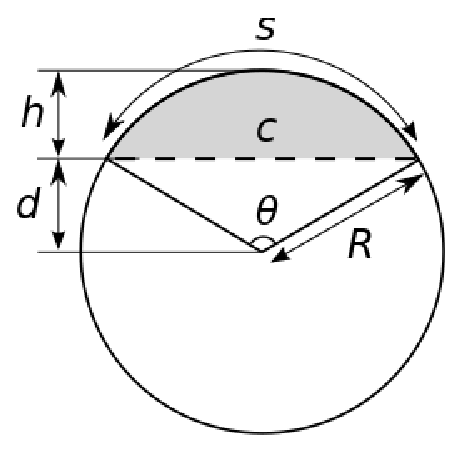
\includegraphics[scale=0.4]{images/circular}
   \caption{Un segmento circular.}
   \label{fig:circular}
\end{figure}

Podría decirse que estos son los primeros pasos de la trigonometría,
desarrollada mucho después por el matemático griego Hiparco.  Los babilonios no
desarrollaron la noción de ángulo, solamente aparecen en los documentos
implícitamente los triángulos rectángulos. 

De los textos encontrados resulta evidente que los babilónicos conocían la
proporcionalidad entre los lados de triángulos semejantes, sabían cómo calcular
áreas de triángulos y trapecios y volúmenes de prismas y cilindros. Los textos
nos muestran que los babilónicos disponían de una técnica medio geométrica y
medio algebraica, que les permitió manipular eficientemente ecuaciones lineales
y cuadráticas. Esta técnica es muy similar a la que nos encontraremos en uno de
los libros de Euclides, escrito aproximadamente en el año 300 a. C.
Intentaremos describir brevemente esta técnica de los babilónicos y para esto
seguiremos la presentación del primer volumen del tratado de Babini y Rey
Pastor~\cite{BabiniReyPastor1,BabiniReyPastor2}.  Supongamos que se tiene un
cuadrado como el que vemos en la figura~\ref{fig:babilonios}. 
\begin{figure}
   \centering
   \includegraphics[scale=0.4]{images/babilonios}
   \caption{La técnica de los babilónicos.}
   \label{fig:babilonios}
\end{figure}
Si el segmento AB mide $a$ y AD mide $b$, entonces AC mide $a+b$ y BD mide
$a-b$. Si O es el centro de simetría del segmento AC, entonces AO y OC son
ambos iguales a $\frac12(a+b)$ y además DO y OB son ambos iguales a
$\frac12(a-b)$. El cuadrado de la figura~\ref{fig:babilonios} puede
descomponerse en cuadrados y rectángulos y de estas descomposiciones podemos
obtener las siguientes fórmulas:
\begin{align*}
	(a+b)^2 &= a^2+b^2+2ab,\\
	(a-b)^2+2ab &= a^2 + b^2,\\
	(a+b)(a-b) &= a^2-b^2,\\
	(a+b)^2 &= 4ab+(a-b)^2,
\end{align*}
fórmulas que los babilónicos usaron en la resolución de problemas. Si $c$ es la medida de la hipotenusa del triángulo
DCM, entonces obtenemos también que 
\[
	c^2\pm 2ab=(a\pm b)^2,
\]
fórmula que no es otra cosa sino una versión del teorema de Pitágoras. La
fórmula $(a+b)^2=(a-b)^2+4ab$ nos lleva casi inmediatamente a la regla de
construcción de ternas pitagóricas que mencionamos anteriormente: simplemente
debemos tomar $a=m^2$, $b=n^2$ y luego 
\[
	(m^2-n^2)^2+(2mn)^2=(m^2+n^2)^2.
\]


